\chapter{Introduction}
\label{chp:1}
\epigraph{Research is what I'm doing when I don't know what I'm doing.}{Wernher von Braun}

The Brazilian aerospace industry is strongly represented in the world by Embraer (in portuguese \textit{Empresa Brasileira de Aeron\'autica}). This company, through its aircraft, is one of the leading exporters of Brazil, with the highest added value product. Examples of aircraft produced by Embraer are the executive Legacy 600 (\autoref{fig:e600}), the military Super Tucano (\autoref{fig:etucano}) and the commercial E-jets  (\autoref{fig:ejets}).

\begin{figure}[H]%
\caption[Embraer aircrafts]{Embraer aircrafts:
\subref{fig:e600} Legacy 600;
\subref{fig:etucano} Super Tucano;
\subref{fig:ejets} E-jets}%
\label{fig:aircrafts}%
\begin{center}
\subfigure[][]{%
\label{fig:e600}%
\begin{minipage}{0.45\textwidth}
\centering
\includegraphics[width=0.8\linewidth]{figs/Embraer_Legacy_600}%
\end{minipage}}
%
\subfigure[][]{%
\label{fig:etucano}%
\begin{minipage}{0.45\textwidth}
\centering
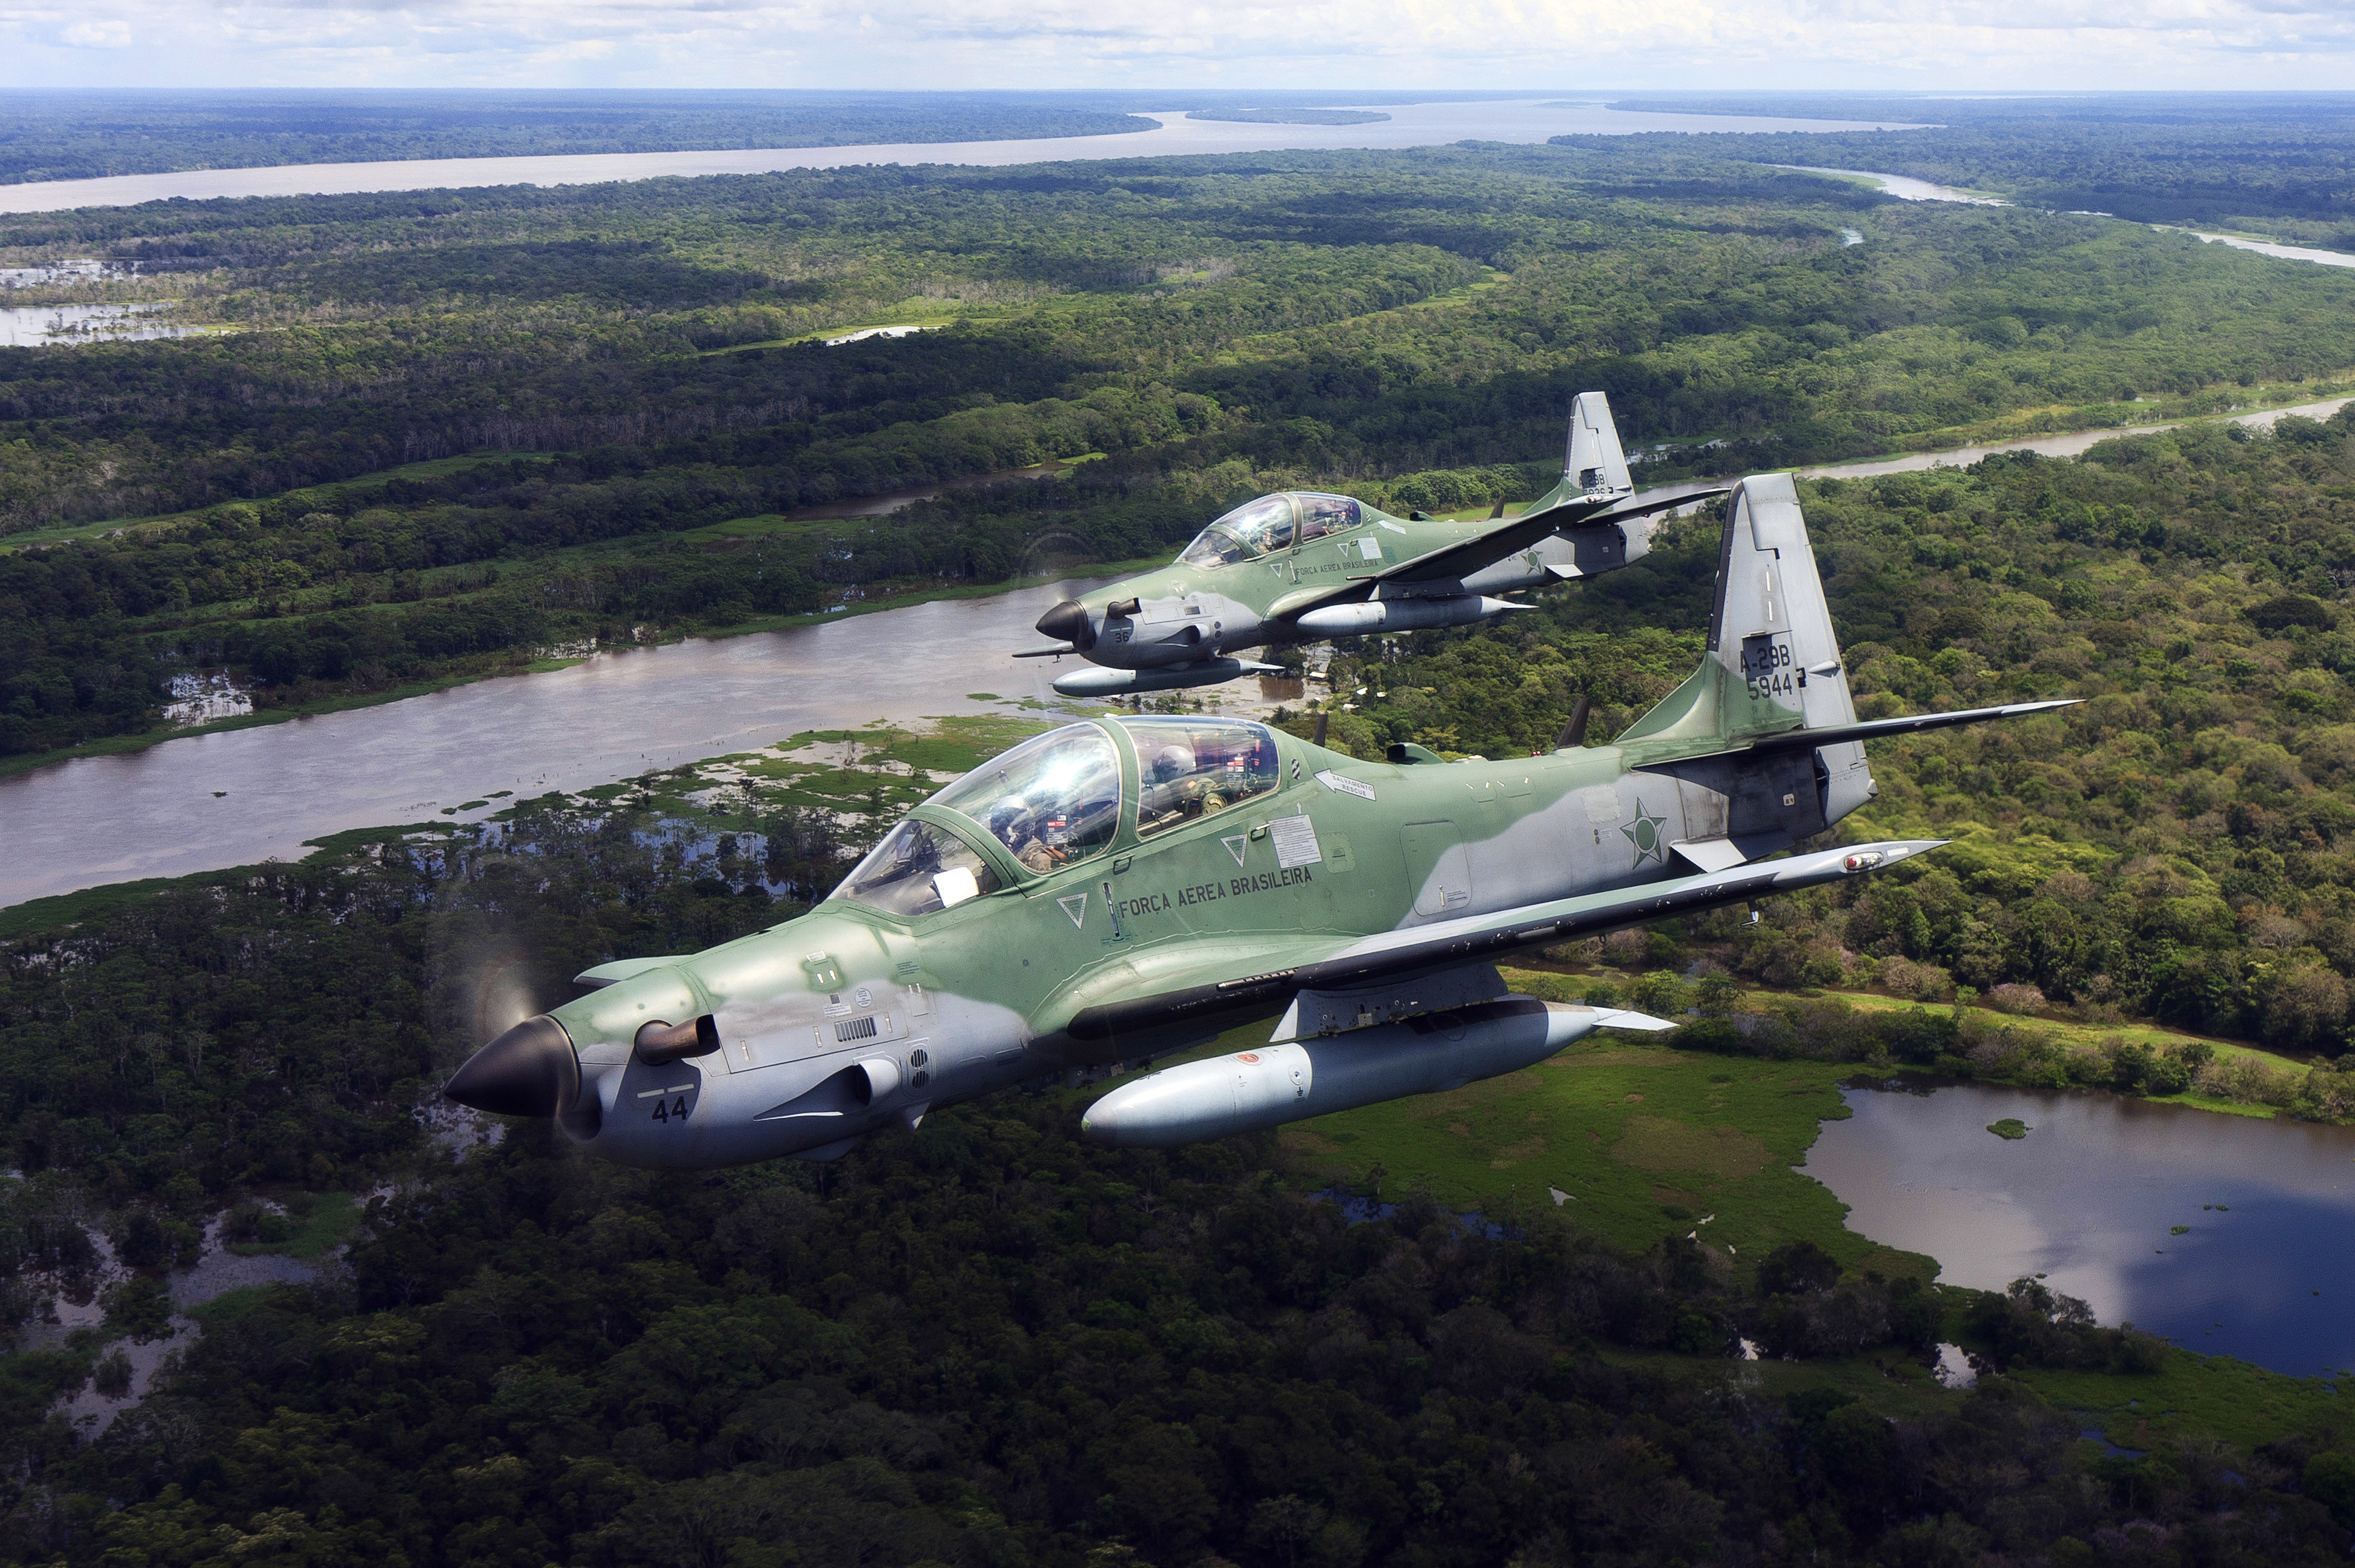
\includegraphics[trim=0 50 0 50, clip, width=0.8\linewidth] {figs/supertucano}
\end{minipage}}\\
\subfigure[][]{%
\label{fig:ejets}%
\begin{minipage}{0.9\textwidth}
\centering
\includegraphics[trim=100 0 100 0, clip, width=0.8\linewidth]{figs/embraerE}
\end{minipage}}%
\end{center}
\vspace{1.5em}
\FONTE{(a) \href{https://es.wikipedia.org/wiki/Embraer_Legacy_600}{Wikipedia: Embraer Legacy 600} (b) \href{https://es.wikipedia.org/wiki/Embraer_EMB_314_Super_Tucano}{Wikipedia: Embraer EMB 314 Super Tucano} (c) \href{http://www.embraercommercialaviation.com}{Embraer Commercial Aviation}}
\end{figure}

Another institution that works with aerospace structures is the National Institute for Space Research (in portuguese \textit{Instituto Nacional de Pesquisas Espaciais} (INPE)). INPE develops satellites for Earth observation, in projects together with other countries such as China, India, and Russia. Examples of satellites developed by INPE are the Data Collection Satellite (SCD-1 \cite{SCD1} and SCD-2, see \autoref{fig:scd}), the China-Brazil Earth Resources Satellite Program (CBERS-1, CBERS-2, CBERS-2B, CBERS-3, CBERS-4, \cite{CBERS}, see \autoref{fig:cbers}) and the Amaz\^onia project (Amaz\^onia-1, \cite{AMAZONIA}, see \autoref{fig:amazonia}).

\begin{figure}[H]%
\centering
\caption[INPE satellites]{INPE satellites:
\subref{fig:scd} SCD-1;
\subref{fig:cbers} CBERS-3;
\subref{fig:amazonia} Amaz\^onia-1}%
\label{fig:satellites}%
\subfigure[]{%
\label{fig:scd}%
\begin{minipage}{0.45\textwidth}
\centering
\includegraphics[trim=5 5 5 5, clip, width=0.4\textwidth]{figs/scd1_2}
\end{minipage}}
%
\subfigure[]{%
\label{fig:cbers}%
\begin{minipage}{0.45\textwidth}
\centering
\includegraphics[width=0.7\textwidth]{figs/CBERS4}
\end{minipage}}\\
\subfigure[]{%
\centering
\label{fig:amazonia}%
\begin{minipage}{\textwidth}
\centering
\includegraphics[width=0.7\textwidth]{figs/amazonia}
\end{minipage}}%
\vspace{1.5em}
\FONTE{(a) \href{http://www.inpe.br/scd1/site_scd/scd1/osatelite.htm}{INPE: \textit{Satélite SCD-1}} (b) \href{http://www.cbers.inpe.br/sobre_satelite/lancamento_cbers4.php}{INPE: \textit{Lançamento CBERS-4}} (c) \href{http://www.inpe.br/amazonia-1/sobre_satelite/}{INPE: \textit{Miss\~ao Amazonia-1}}}
\end{figure}

The design of an adequate computer model for the structural analysis is fundamental in the development and construction process of engineering structures.  Computer-Aided Engineering (CAE) is the extensive use of computer software to assist in engineering analysis tasks, including Finite Element Analysis (FEA), Computational Fluid Dynamics, Multibody Dynamics, and optimization of products or processes. Some examples of computer software for solving problems by the FEA are Algor, Abaqus, ANSYS, COSMOS/M, T-STRUDL, MARC, MSC/NASTRAN, NISA, Pro/MECHANICA, SAP2000, and STARDYNE \cite{logan2011first}. Those programs are widely used in the designing and analysis processes of structures in aerospace industry \cite{Birtles1983}. For example, Embraer and INPE adopted the NASTRAN, which performs different engineering analysis, such as static, dynamic, and thermal analysis.

Aerospace structures are critical systems. Failures in structures would cause catastrophic consequences, with human and material losses. Hence, it is essential to have the capability of detecting damages in an early stage, with accuracy, and safely. This detection should help to repair or rehabilitate a structure before it has major damages.

Structural health monitoring (SHM) is an important application of the field of System Identification that combines the advances of sensing technologies with theories and techniques for nondestructive damage detection (NDD). One relevant capability of SHM is its ability to monitor a structure during its operation. 

In Brazil, efforts are being made to develop a Brazilian technology in the solution of practical problems of great interest to the aerospace industry, such as Structural Damage Identification.

\section{Damages}

Damages can be defined as changes to the material or geometric properties of a structure, including changes in the boundary conditions and the system connectivity, which affect its current or future performance. The damage identification is linked to a comparison of two different states of a structure, one of which is the initial state, named undamaged, and the other is the current structural response under a forcing term. The existence of damage does not imply that the system/structure losses all its functionality, but rather that it does not operate in its standard manner.

Examples of damages are, among others, cracks, local plasticity, delamination and debonding in composite materials.

A damage can be categorized in accidental damage, fatigue damage, or environmental damage \cite{baaran2009, venterink2017frequency}. Damages associated with fatigue or corrosion in metals can accumulate incrementally over periods of time. For composites, inspection of fatigue and environmental damages are often not required, if proper design precautions were taken.

In short time-scales, accidental damages can be the result of scheduled discrete events such as aircraft landings, or unscheduled events, such as bird-strikes in aircraft or natural phenomena hazards.

As damages increase, the system/structure operation will be no longer acceptable to the user, i.e., a failure will occur. An unpredicted structural failure can cause catastrophic loss of economic value and human life.

Damages in aerospace structures can be categorized according to their severity \apud{ilcewicz2006composite}{baaran2009}:

\begin{enumerate}
    \item Allowable damage that may go undetected by scheduled or direct field inspection, for example, allowable manufacturing defects, but also non-allowable damage: Barely Visible Impact Damage (BVID), e.g., damage caused by debris or hailstones.
    \item Damage detected by scheduled or direct field inspection at specified intervals, e.g. exterior skin damage, or interior stringer blade damage.
    \item Obvious damage detected within a few flights by operations, e.g. accidental damage to the lower fuselage, or lost bonded repair patch.
    \item Discrete source damage immediately known by the pilot limiting flight maneuvers, e.g. rotor disk cut through the fuselage or severe rudder lightning damage.
    \item Severe damage created by anomalous ground or flight events, e.g. bird-strike, maintenance jacking incident, propeller mishap.
\end{enumerate}

\section{Structural damage identification}
The Structural Damage Identification (SDI) process involves the conjunction of five disciplines \cite{farrar2010introduction, Farrar2007c}:

\begin{description}[style=sameline]
\item[Structural Health Monitoring] SHM performs a global damage identification for aerospace, civil and mechanical engineering infrastructure, and it can be performed off-line as well as on-line.  On-line refers to the monitoring during operation of the system or structure, while off-line refers to the monitoring during maintenance;
\item[Condition Monitoring] Condition Monitoring is analogous to SHM, but in rotating and reciprocating machinery;
\item[Non-Destructive Evaluation] Non-Destructive Evaluation carried out off-line in a local manner after the damage has been located;
\item[Statistical Process Control] Statistical Process Control is based on process and uses a variety of sensors to monitor changes in a process;
\item[Damage Prognosis] Damage Prognosis evaluates the damage evolution and predicts the remaining useful life of a system.
\end{description}

All these processes involve the observation of a structure or a mechanical system for a period, by mean of periodically spaced measurements; the extraction of damage-sensitive features from the measurements; and the analysis of these features to determine the current state of the structural health.

The process of damage identification involves four steps:

\begin{description}[style=sameline]
\item[Operational Evaluation] Gives details of the implementation of the process, such as possible failure modes, operational and environmental conditions, and limitations related to data acquisition.
\item[Data Acquisition] Defines the quantities to be measured, the amount of data to be saved, and how the data will be acquired (which and how many sensors will be used, and where the sensors will be placed). Also, defines the data fusion and cleansing, that determine which data is necessary and useful in the feature extraction process.
\item[Feature Extraction] Identifies damage sensitive parameters from measured data.
\item[Classification] Performs the comparison between the damaged and undamaged states and quantifies the damage.
\end{description}

An ideal robust damage identification scheme should be able to detect a damage at a very early stage, locate the damage within the sensor resolution, provide an estimate of the extent or severity of the damage, and predict the remaining useful life of the structural component when the damage is identified. The identification should be independent of changes in the operational and environmental conditions. The method should also be well suited to automation and should be independent of human judgment and ability \cite{Doebling1996}.

\subsection{Classification of the Structural Damage Identification methods}
Damage identification methods can be classified in different ways: according to their performance, and to whether they are local or global, model or non-model based, and whether they use a baseline or not. 

\textbf{Performance}
The damage identification process for a system of a structure can by classified attending five levels of performance \cite{Rytter1993,Sohn2004, Worden2004, Worden2007}:

\begin{description}[style=sameline]
\item[Level 1: Detection] Verification of the presence of damage in a structure
\item[Level 2: Location] Determination of the location of the damage
\item[Level 3: Type] Determination of the type of the damage
\item[Level 4: Extension] Estimation of the extent and severity of the damage
\item[Level 5: Prognosis] Prediction of the remaining service life of the structure
\end{description}

The first four levels (Detection, Location, Type, and Extension) are related to the damage diagnosis, while the fifth step is related to the damage prognosis. Increasing the level implies a higher degree of complexity and a greater necessity of mathematical models.

\textbf{Local or global methods}

This classification is related to the inspection domain concerning the structure \cite{Fritzen2009}:

\begin{description}[style=sameline]
\item[Local] Concentrated on a specific part of the structure.
\item[Global] The whole structure is analyzed.
\end{description}

Local methods are usually considered to be more sensitive than global methods. Local methods are capable of detecting small damages, while global ones can identify only relatively severe damages. However, local methods are applicable with a prior knowledge of the location of a damaged area of the structure.

\textbf{Model or non-model based approach}

Methods can also be classified on model and non-model based:

\begin{description}[style=sameline]
\item[Non-model based] The response of the structure in service is compared with results of a reference measurement previously acquired. Deviations in damage sensitive parameters are used to identify damage.
\item[Model based] The response is compared with the results obtained from an analytical or numerical model.
\end{description}

Advantages of model based over the non-model based techniques include the possibility of the former to be easily extended to provide information about the severity of the detected damage and can be used to account for environmental or operational variations (e.g. temperature, boundary conditions, etc.). Disadvantages include the difficulty in obtaining an accurate model representation of complex structures, and its limited applicability for \textit{in situ} monitoring, due to their computational cost.

\textbf{Baseline or non-baseline}

The process of identifying a damage requires the comparison of two states, one of them being the undamaged reference. Therefore, methods can also be classified according to whether  a baseline is used or not \cite{Worden2007}:

\begin{description}[style=sameline]
\item[Baseline] The response of the structure, measured at an earlier stage, is usually utilized as a baseline to distinguish between the damaged and undamaged states.
\item[Non-baseline] The response is compared with a state of the structure assumed to have a normal behavior (e.g. a smooth pattern or linear-elastic response). The system is in this case classified as damaged when the response deviates from the expected behavior.
\end{description}

SDI can be treated as two complementary approaches \cite{Montanari2014}:
\begin{description}[style=sameline]
\item[Inverse problem] This approach typically uses a model of the structure and tries to relate changes in measured data from the structure to changes in the model \cite{friswell2007damage}. Locally linearized models are sometimes used to make the analysis simpler. The behavior of the real structure is compared to the corresponding model, through optimization algorithms.
\item[Pattern recognition problem] This approach follows the concepts of the Pattern Recognition (PR) problem \apud{schalkoff1992pattern}{Montanari2014}
\end{description}

\section{Literature overview of techniques for Structural Damage Identification}
\label{chap:state}

A high amount of Non-Destructive Evaluation (NDE) techniques can be used for damage identification. Most of them can only be applied off-line. Thus, only a minor quantity of these techniques can be used in an SHM system.

\autoref{fig:methods} shows a scheme of these techniques (first three lines), that include the Structural Vibration (SV) and Electromechanical Impedance (EMI) techniques which primarily rely on standing wave patterns. Another group, including the higher frequency Acoustic Emission (AE), Acousto-Ultrasonic (AU), and Ultrasonic Testing (UT), employ traveling wave characteristics.

SV and EMI provide results that are relatively easy to interpret. More complex structures can be analyzed with these methods, allowing to explore outright a relatively large area. However, in these methods the limited frequency range causes a limited resolution, and only relatively severe damage, such as delaminations, can be identified.

AE, AU and UT can all detect small damages, such as cracks. For this reason, these wave based technologies are more frequently used for aircraft applications \cite{Staszewski2009,Diamanti2010}. However, the interpretation of the data is more complicated than with SV and EMI, especially in the case of non-flat or composite structures \cite{Dalton2001}.

\begin{sidewaysfigure}
\caption{Overview of damage identification methods. The branch of vibration-based methods is detailed with different features and classifiers used in the literature}
\label{fig:methods}
\centering
\vspace{1em}
\resizebox{\textwidth}{!}
{
\includegraphics{images/chapter1_methods.tikz}
}
\vspace{1em}
{\footnotesize SOURCE: Adapted from \cite{Ooijevaar2014}}
\end{sidewaysfigure}

\begin{table}[H]
    \caption{Dynamics based NDE technologies}
    \label{tab:my_label}
    \centering
    \footnotesize
    \begin{tabular}{cccccc}
        \toprule
        Technology & \specialcell{Frequency\\range [Hz]} & \specialcell{Actuation\\approach} & \specialcell{Sensitivity\\to damage} & \specialcell{Ease of data\\interpretation} & \specialcell{Applicability\\for SHM} \\
        \midrule
         SV & $10^0 - 10^4$ & Active / passive & ++ & +++ & ++++ \\
         EMI & $10^3 - 10^5$ & Active & +++ & +++ & ++++ \\
         AE & $10^4 - 10^6$ & Passive & ++++ & ++ & +++ \\
         AU & $10^4 - 10^6$ & Active & ++++ & + & ++++ \\
         UT & $10^5 - 10^7$ & Active & +++++ & ++ & + \\
         \bottomrule
    \end{tabular}
    \FONTE{Adapted from \cite{Ooijevaar2014}}
\end{table}

Vibration-based SHM and damage detection techniques receive a great attention in the aeronautic engineering field \cite{Liu2012}. A good system for SHM can increase the efficiency of structural maintenance, reducing the cost and enhancing the reliability of the structures \cite{de2016shm}.

\subsection{Methods based on structural vibration for structural damage identification}
\label{sec:methods}

The literature dealing with SV methods is vast. Different methods are classified depending on their approach, e.g., frequency changes, mode shape changes, dynamically measured flexibility, matrix update methods, nonlinear methods, Neural Networks-based methods, and other methods. These kind of methods are the subject of books \cite{Balageas2006,Boller2009}, doctoral theses \cite{Ooijevaar2014,de2016shm}, and review papers, some of them on specific topics (composite materials, strain based methods, nonlinear methods) \cite{Doebling1996,Doebling1998,Zou2000,Sohn2004,Carden2004,Montalvao2006,Fassois2007,Worden2008,Jhang2009,Fritzen2009,Li2010,Fan2011}. \autoref{fig:methods} summarizes the principal damage sensitive features and classifiers found in the literature on the Vibration-based Damage Identification methods category. These methods can be divided into three principal areas: time, frequency and modal domains. \autoref{tab:features} shows an overview of these features, while \autoref{tab:alldomains} in \autoref{app:A} shows a more detailed list of classifiers associated with the features.

\citeonline{Doebling1998} affirmed that sufficient evidence exists to promote the use of measured vibration data for damage identification in structures, using forced-response tests and long-term monitoring of ambient signals.

\begin{table}[H]
    \caption{Overview of the vibration based damage features}
    \label{tab:features}
    \centering
    \scriptsize
    \begin{tabular}{L{0.2\textwidth}L{0.2\textwidth}L{0.2\textwidth}L{0.2\textwidth}}
        \toprule
         Time & Time-frequency & Frequency & Modal \\
         \midrule
         Time response / waveform & Wavelet transform & Fourier / power spectra & Natural frequencies \\
         Statistical time series analysis & Hilbert transform & Frequency response function & Mode shape \\
         & Hilbert-Huang transform & Frequency response function curvature & Mode shape curvatures \\
         & & Mechanical impedance & Modal damping \\
         & & Transmissibility function & Dynamic stiffness \\
         & & Anti-resonances & Dynamic flexibility \\
         & & Higher harmonics (nonlinear) & Updating methods \\
         & & Modulation (nonlinear)\\
         \bottomrule
    \end{tabular}
    \FONTE{Adapted from \cite{Ooijevaar2014}}
\end{table}

\subsection{Metaheuristics applied to structural damage identification}

\autoref{tab:intelligence} shows a compilation of papers where the SDI problem is approached using different Computational Intelligence techniques. They can be divided into five groups: neural network techniques, support vector machine, fuzzy inference, metaheuristic algorithms, and hybrid techniques. Among them, the formulation of the SDI problem as a constrained optimization problem is typically considered the most effective strategy \cite{Yu2011}.

Some authors have used the classic Genetic Algorithm (GA) for solving the Damage Identification problem. For instance, \citeonline{Mares1996} located and quantified damages in truss and beam structures; \citeonline{Borges2007} identified damages in a framed structure; and recently, \citeonline{Boonlong2014} used Cooperative Coevolutionary Genetic Algorithm as the optimizer for the vibration-based damage detection in beams.

Other classical metaheuristics have also been used for this purpose. A continuous variant of Ant Colony Optimization (ACO) was used by \citeonline{Yu2011} to detect single and multiple damages on 2 and 3-storey building models; they suggested the use of hybrid approaches of ACO to improve the results. In \citeonline{Braun2015}, different versions of ACO, as well as hybrid variants using HJ, were used to detect damages on a damped spring-mass system.

A combination of a self-configurable Particle Swarm Optimization (PSO) with the Nelder-Mead (NM) algorithm has also been used for optimal localization of sensors for health monitoring \cite{rao2007optimal}. In \citeonline{abdalla2009particle}, PSO was also applied in the solution of the inverse problem of structural damage identification using a cantilever beam model. The hybrid PSO-simplex (PSOS) was used in two structural damage identification problems with noisy and incomplete data, in the frequency domain. \citeonline{begambre2009hybrid} used Latin hypercube sampling and PSO for an experimental verification of the structural damage detection process. \citeonline{kang2012damage} proposed an immunity enhanced particle swarm optimization (IEPSO) algorithm for damage detection, which was used for a simply supported beam, and on a plane truss structure. Also, \citeonline{VakilBaghmisheh20122217} hybridized PSO with NM for crack detection in cantilever beams.

Recently, the novel Bird Mating Optimizer (BMO) was used in \citeonline{Zhu2017} for identifying structural damages using the minimization of the differences between the measured and calculated natural frequencies and correlation function acceleration vector of damaged and undamaged structures. This method was used for identifying damages on a planar frame structure, and a three connected shear building.

This topic has served to present new metaheuristics. For example, the Big Bang-Big Crunch (BBC), in \citeonline{Tabrizian2013}, is used to identify damages in beam bridges, a Belgian truss, and a two-story two-bay frame. In their work, this algorithm minimizes an objective function using complete and incomplete modal data, with and without noise. In \citeonline{Yu2014}, single and multiple damage cases are detected in a simulated 4-storey benchmark frame structure, and in a 2-storey rigid frame, using the global Artificial Fish Swarm Algorithm (GAFSA). Also, an experimental laboratory study on damage detection was performed in a 3-storey building model, with four damage patterns. \citeonline{Ding20161} presented the quick ABC (QABC), an artificial bee colony (ABC) algorithm with hybrid search strategy based on modal data. QABC is applied in the damage identification of a truss and a plate.

{
\scriptsize
\centering
\renewcommand{\arraystretch}{0.9}
\begin{longtable}{L{8.2cm}L{5.8cm}}
\caption{Literature overview of Computational Intelligence methods used for SDI}
\label{tab:intelligence}
\endfirsthead
\multicolumn{2}{c}%
{\tablename\ \thetable\ -- \textit{Continued from previous page}} \\
\toprule
\endhead
\midrule \multicolumn{2}{r}{\textit{Continued on next page}} \\
\endfoot
\midrule
\endlastfoot
\toprule
\multicolumn{2}{l}{\textbf{Neural networks}}\\
\midrule
Iterative Neural Network (INN) & \cite{Chang2000}\\
Backpropagation NN (BP-NN) & \cite{Zang2001}\newline \cite{Yam2003a}\newline \cite{Pawar2006}\newline \cite{Mehrjoo2008} \newline \cite{Chiwiacowsky2008}\\
Multilayer Neural Network (MNN) & \cite{Huang2001}\\
Extended Kalman Filter Trained Neural Network (EKFNN) & \cite{Jin2016}\\
\midrule
\multicolumn{2}{l}{\textbf{Support Vector Machine (SVM)}}\\
\midrule
Hyper-Solution SVM (HSVM) & \cite{Candelieri2014}\\
\midrule
\multicolumn{2}{l}{\textbf{Fuzzy}}\\
\midrule
Fuzzy Clustering (FC) & \cite{Silva2008}\\
Fuzzy Logic System (FLS) & \cite{Chandrashekhar2009}\\
\midrule
\multicolumn{2}{l}{\textbf{Metaheuristics}}\\
\midrule
Genetic Algorithm (GA) & \cite{Boonlong2014} \newline \cite{Borges2007} \newline \cite{Chou2001} \newline \cite{Gomes2008} \newline \cite{Mares1996}\\
Improved PSO (IPSO) & \cite{Yu2008}\\
Tabu Search (TS) & \cite{Arafa2010}\\
Continuous ACO (CnACO) & \cite{Yu2011}\\
Ant Colony Optimization (ACO) & \cite{Majumdar2012} \newline \cite{Yu2011}\\
Swarm Intelligence (SI) & \cite{Yu2012} \\
Particle Swarm Optimization (PSO) & \cite{Mohan2013} \newline \cite{Seyedpoor2012}\\
Big Bang-Big Crunch (BB-BC) & \cite{Tabrizian2013}\\
Simulated Annealing (SA) & \cite{Kourehli2013}\\
Differential Evolution (DE) & \cite{Fu2014} \newline \cite{Seyedpoor2015} \newline \cite{Seyedpoor2015a}\\
Charged System Search (CSS) & \cite{kaveh2015improved}\\
 Multi-Swarm Fruit Fly Optimization Algorithm (MFOA) & \cite{li2015multi} \\
Global Artificial Fish Swarm Algorithm (GAFSA) & \cite{Yu2014} \\
Rank-based Ant System (RAS) & \cite{Braun2015}\\
Ant System with Heuristic Information (ASH) & \cite{Braun2015}\\
Elitist Ant System (EAS) & \cite{Braun2015}\\
Firefly Algorithm (FA) & \cite{Pan2015} \\
Cyclical parthenogenesis algorithm (CPA) &
\cite{Kaveh2017} \\
\midrule
\multicolumn{2}{l}{\textbf{Hybrid algorithms}}\\
\midrule
Genetic Algorithm + Conjugated Gradient Method (GA-CGM) & \cite{Chiwiacowsky2006} \newline \cite{Chiwiacowsky2006b}\\
Genetic Algorithm + Levenberg-Maquardt (GA-LM) &\cite{He2006} \\
Genetic Fuzzy System (GFS) & \cite{Pawar2007}\\
Simulated Annealing Genetic Algorithm (SAGA) & \cite{Kokot2009} \\
Genetic Algorithm and Particle Swarm Optimization (GA-PSO) & \cite{Sandesh2010}\\
Ant System with Heuristic Information + Hooke-Jeeves (ASH-HJ) & \cite{Braun2015}\\
PSO with Nelder-Mead (PSO-NM) & \cite{Chen2015}\\
Multi-Particle Collision Algorithm with Hooke-Jeeves (MPCA-HJ) & \cite{HernandezTorres2015b}\\
$q$-Gradient with Hooke-Jeeves ($q$G-HJ) & \cite{HernandezTorres2015} \\
Firefly Algorithm / Genetic Algorithm & \cite{khatir2016multiple}\\
Quick Artificial Bee Colony algorithm (QABC) & \cite{Ding20161}\\
Particle Swarm Inspired
Multi-Elitist Artificial Bee Colony (PS-MEABC) & 
\cite{Fatahi2017}\\
\bottomrule
\end{longtable}
}

\subsection{Gaps found in the literature}

As discussed in \autoref{sec:methods}, many damage identification techniques have been proposed in the literature. However, their practical application can be difficult \cite{Doebling1998,Ooijevaar2014}.

There are uncertainties in damage identification \cite{xu2017smart}, mainly caused by:
%Smart Civil Structures
\begin{itemize}
    \item Methodology errors:
    \vspace{0.5em}
    \begin{itemize}
    \item Limitations of the damage identification methods;
    \end{itemize}
    \vspace{-0.5em}
    \item Modeling errors:
    \vspace{0.5em}
    \begin{itemize}
    \item Inaccuracy in the discretization of the FE model;    
    \item Uncertainties in the geometry and boundary conditions;
    \item Variations in material properties;
    \item Operational and environmental variability;
    \end{itemize}
    \vspace{-0.5em}
    \item Measurement errors:
    \vspace{0.5em}
    \begin{itemize}
    \item Errors in the measured signals, caused by noise, or by procedures in the measurements;    
    \item Errors in the post-processing techniques;
    \end{itemize}
\end{itemize}

Some issues that need to be solved to enable the actual practice of these methods are summarized below:

\begin{description}[style=sameline]
\item[Lack of robustness] None of the methods solves all problems for all structures.

\item[Occurrence of False alarms] One of the main challenges in damage identification is the development of methods that provide a high detection probability, without false alarms. There are two types of false damage identification: \textit{false-positive}, when a intact element is identified as damaged, and a \textit{false-negative}, that is a failure in identifying damaged elements. A false-negative can cause serious life and safety consequences, while a false-positive causes a decrease in the reliability of the method.

\item[Low-performance level] Most of the methods attends the first two levels of performance (detecting and locating damage), but they are limited in their capability to achieve a prognosis, as well as in classifying the type and severity of the damage \cite{Ooijevaar2014}. The prognosis is the prediction of the remaining lifetime of the structure through the analysis of the damage evolution. It represents an important step for the development of autonomous systems for monitoring the structural health.

\item[Low complexity structures] Most of the methods deals with relatively low complexity structures (simple concrete or metallic structures, or relatively simple composite beams and plates structures). These structures are typically well-defined, or the damage scenario is created artificially. It is necessary to focus on more specific applications, such as real life and industrial structures like air-frames, bridges, and other long design life structures with life-safety or economic implications.

\item[No integration with engineering software] CAE software help in the task of modeling and analyzing structures. Among the papers revised, the use of these computer programs is scarcely mentioned.

\item[No operational and environmental variability] In real applications, the operational and environmental conditions, such as temperature and wind, could mask or modify the effects of the damages. Good approaches should have the capability of to separate their effects.

\item[Integrated sensor and network] Another problem is related to the optimal quantity and location of the sensors because they are expensive. Also, obtaining many signals increases the computational cost, and could add errors due to the inherent noise of the sensors and some possible external noises.

\item[Cooperation] Due to the magnitude of the projects, more cooperation is required between academia and industry.
 
\end{description}

More detailed discussions on these problems are provided by \citeonline{farrar2007introduction} and \citeonline{boller2013structural}.

In this thesis, the SDI will be defined as an inverse problem and solved as an optimization problem.

\section{Research objective}

The main objective of this thesis is:

\begin{quote}
To develop hybrid metaheuristics for identifying damages on structures modeled in FORTRAN and NASTRAN, using a hierarchical approach.
\end{quote}

This work will contribute to the improvement of the Multi-Particle Collision Algorithm and the $q$-gradient method, to the creation of hybrid algorithms, and to their application in the development of a tool to assist the implementation of structural health monitoring technology in aerospace structures.

\subsection{Tasks}

Specific tasks and sub-tasks were also defined to accomplish the main objective:

\begin{enumerate}
\item Perform a literature review on methods for Damage Identification;
\item Perform modifications in the Multi-Particle Collision Algorithm, for performance improvement;
\vspace{0.5em}
\begin{enumerate}
\item Modificate functions for improving the exploration and the exploitation of the algorithm;
\end{enumerate}
\item Develop hybrid algorithms based on MPCA and $q$-gradient, using concepts derived from the Opposition Based Learning, and the direct-search method Hooke-Jeeves;
\item Identify damages on structures with different complexities implemented in FORTRAN;
\vspace{0.5em}
\begin{enumerate}
\item Model structures with different types and complexities in FORTRAN;
\item Identify damages on structures implemented using finite elements on FORTRAN using hybrid algorithms;
\end{enumerate}
\item Identify damages on structures with different complexities modeled on NASTRAN;
\vspace{0.5em}
\begin{enumerate}
\item Model structures with different types and complexities in NASTRAN;
\item Identify damages on structures modeled on NASTRAN using hybrid algorithms;
\end{enumerate}
\item Identify damages on structures modeled on NASTRAN using a hierarchical approach;
\vspace{0.5em}
\begin{enumerate}
\item Identify damages on structures with medium complexity, through the hierarchical approach, using hybrid algorithms.
\end{enumerate}
\end{enumerate}

\section{Outline}

This thesis is structured into ten chapters, including introduction and conclusions, and three appendixes, organized as follow:

\begin{description}[style=sameline,labelindent=1cm]
\item [\fullref{chp:1} (this chapter)] In this chapter, the research objective and main tasks are defined.
\item [\fullref{chp:3}] 
\item [\fullref{chp:4}] In this chapter, the transient response analysis of structures is presented as the forward model. The mathematical definition and the numerical solution of direct and modal methods is summarized. Then, the Finite Element Method is introduced and presented the explanation of how it is applied in computing the model of systems with springs, and structures with bars and beams.
\item [\fullref{chp:5}]
\item [\fullref{chp:6}]
\item [\fullref{chp:7}]
\item [\fullref{chp:8}]
% \item [\fullref{chp:9}]
\item [\fullref{chp:10}]
\item [References]
\item [\fullref{app:A}] This appendix presents the main features and classification approaches found in the literature, with an exhaustive bibliographic revision.
\item [\fullref{vita}] This annex presents the vita of the author of this thesis, including full papers on journals, national and international congresses, that directly or indirectly contributed to the doctoral thesis.

\end{description}
